\documentclass[11pt]{article}
\usepackage{float}
% NOTE: Add in the relevant information to the commands below; or, if you'll be using the same information frequently, add these commands at the top of paolo-pset.tex file. 
\newcommand{\name}{Agustín Esteva}
\newcommand{\email}{aesteva@uchicago.edu}
\newcommand{\classnum}{270}
\newcommand{\subject}{Complex Variables}
\newcommand{\instructors}{Robert Fefferman}
\newcommand{\assignment}{Problem Set 4}
\newcommand{\semester}{Spring 2025}
\newcommand{\duedate}{5-01-2025}
\newcommand{\bA}{\mathbf{A}}
\newcommand{\Ind}{\text{Ind}}

\newcommand{\bB}{\mathbf{B}}
\newcommand{\bC}{\mathbf{C}}
\newcommand{\bD}{\mathbf{D}}
\newcommand{\bE}{\mathbf{E}}
\newcommand{\bF}{\mathbf{F}}
\newcommand{\bG}{\mathbf{G}}
\newcommand{\bH}{\mathbf{H}}
\newcommand{\bI}{\mathbf{I}}
\newcommand{\bJ}{\mathbf{J}}
\newcommand{\bK}{\mathbf{K}}
\newcommand{\bL}{\mathbf{L}}
\newcommand{\bM}{\mathbf{M}}
\newcommand{\bN}{\mathbf{N}}
\newcommand{\bO}{\mathbf{O}}
\newcommand{\bP}{\mathbf{P}}
\newcommand{\bQ}{\mathbf{Q}}
\newcommand{\bR}{\mathbf{R}}
\newcommand{\bS}{\mathbf{S}}
\newcommand{\bT}{\mathbf{T}}
\newcommand{\bU}{\mathbf{U}}
\newcommand{\bV}{\mathbf{V}}
\newcommand{\bW}{\mathbf{W}}
\newcommand{\bX}{\mathbf{X}}
\newcommand{\bY}{\mathbf{Y}}
\newcommand{\bZ}{\mathbf{Z}}
\newcommand{\Vol}{\text{Vol}}

%% blackboard bold math capitals
\newcommand{\bbA}{\mathbb{A}}
\newcommand{\bbB}{\mathbb{B}}
\newcommand{\bbC}{\mathbb{C}}
\newcommand{\bbD}{\mathbb{D}}
\newcommand{\bbE}{\mathbb{E}}
\newcommand{\bbF}{\mathbb{F}}
\newcommand{\bbG}{\mathbb{G}}
\newcommand{\bbH}{\mathbb{H}}
\newcommand{\bbI}{\mathbb{I}}
\newcommand{\bbJ}{\mathbb{J}}
\newcommand{\bbK}{\mathbb{K}}
\newcommand{\bbL}{\mathbb{L}}
\newcommand{\bbM}{\mathbb{M}}
\newcommand{\bbN}{\mathbb{N}}
\newcommand{\bbO}{\mathbb{O}}
\newcommand{\bbP}{\mathbb{P}}
\newcommand{\bbQ}{\mathbb{Q}}
\newcommand{\bbR}{\mathbb{R}}
\newcommand{\bbS}{\mathbb{S}}
\newcommand{\bbT}{\mathbb{T}}
\newcommand{\bbU}{\mathbb{U}}
\newcommand{\bbV}{\mathbb{V}}
\newcommand{\bbW}{\mathbb{W}}
\newcommand{\bbX}{\mathbb{X}}
\newcommand{\bbY}{\mathbb{Y}}
\newcommand{\bbZ}{\mathbb{Z}}

%% script math capitals
\newcommand{\sA}{\mathscr{A}}
\newcommand{\sB}{\mathscr{B}}
\newcommand{\sC}{\mathscr{C}}
\newcommand{\sD}{\mathscr{D}}
\newcommand{\sE}{\mathscr{E}}
\newcommand{\sF}{\mathscr{F}}
\newcommand{\sG}{\mathscr{G}}
\newcommand{\sH}{\mathscr{H}}
\newcommand{\sI}{\mathscr{I}}
\newcommand{\sJ}{\mathscr{J}}
\newcommand{\sK}{\mathscr{K}}
\newcommand{\sL}{\mathscr{L}}
\newcommand{\sM}{\mathscr{M}}
\newcommand{\sN}{\mathscr{N}}
\newcommand{\sO}{\mathscr{O}}
\newcommand{\sP}{\mathscr{P}}
\newcommand{\sQ}{\mathscr{Q}}
\newcommand{\sR}{\mathscr{R}}
\newcommand{\sS}{\mathscr{S}}
\newcommand{\sT}{\mathscr{T}}
\newcommand{\sU}{\mathscr{U}}
\newcommand{\sV}{\mathscr{V}}
\newcommand{\sW}{\mathscr{W}}
\newcommand{\sX}{\mathscr{X}}
\newcommand{\sY}{\mathscr{Y}}
\newcommand{\sZ}{\mathscr{Z}}


\renewcommand{\emptyset}{\O}

\newcommand{\abs}[1]{\lvert #1 \rvert}
\newcommand{\norm}[1]{\lVert #1 \rVert}
\newcommand{\sm}{\setminus}


\newcommand{\sarr}{\rightarrow}
\newcommand{\arr}{\longrightarrow}

% NOTE: Defining collaborators is optional; to not list collaborators, comment out the line below.
%\newcommand{\collaborators}{Alyssa P. Hacker (\texttt{aphacker}), Ben Bitdiddle (\texttt{bitdiddle})}

% Copyright 2021 Paolo Adajar (padajar.com, paoloadajar@mit.edu)
% 
% Permission is hereby granted, free of charge, to any person obtaining a copy of this software and associated documentation files (the "Software"), to deal in the Software without restriction, including without limitation the rights to use, copy, modify, merge, publish, distribute, sublicense, and/or sell copies of the Software, and to permit persons to whom the Software is furnished to do so, subject to the following conditions:
%
% The above copyright notice and this permission notice shall be included in all copies or substantial portions of the Software.
% 
% THE SOFTWARE IS PROVIDED "AS IS", WITHOUT WARRANTY OF ANY KIND, EXPRESS OR IMPLIED, INCLUDING BUT NOT LIMITED TO THE WARRANTIES OF MERCHANTABILITY, FITNESS FOR A PARTICULAR PURPOSE AND NONINFRINGEMENT. IN NO EVENT SHALL THE AUTHORS OR COPYRIGHT HOLDERS BE LIABLE FOR ANY CLAIM, DAMAGES OR OTHER LIABILITY, WHETHER IN AN ACTION OF CONTRACT, TORT OR OTHERWISE, ARISING FROM, OUT OF OR IN CONNECTION WITH THE SOFTWARE OR THE USE OR OTHER DEALINGS IN THE SOFTWARE.

\usepackage{fullpage}
\usepackage{enumitem}
\usepackage{amsfonts, amssymb, amsmath,amsthm}
\usepackage{mathtools}
\usepackage[pdftex, pdfauthor={\name}, pdftitle={\classnum~\assignment}]{hyperref}
\usepackage[dvipsnames]{xcolor}
\usepackage{bbm}
\usepackage{graphicx}
\usepackage{mathrsfs}
\usepackage{pdfpages}
\usepackage{tabularx}
\usepackage{pdflscape}
\usepackage{makecell}
\usepackage{booktabs}
\usepackage{natbib}
\usepackage{caption}
\usepackage{subcaption}
\usepackage{physics}
\usepackage[many]{tcolorbox}
\usepackage{version}
\usepackage{ifthen}
\usepackage{cancel}
\usepackage{listings}
\usepackage{courier}

\usepackage{tikz}
\usepackage{istgame}

\hypersetup{
	colorlinks=true,
	linkcolor=blue,
	filecolor=magenta,
	urlcolor=blue,
}

\setlength{\parindent}{0mm}
\setlength{\parskip}{2mm}

\setlist[enumerate]{label=({\alph*})}
\setlist[enumerate, 2]{label=({\roman*})}

\allowdisplaybreaks[1]

\newcommand{\psetheader}{
	\ifthenelse{\isundefined{\collaborators}}{
		\begin{center}
			{\setlength{\parindent}{0cm} \setlength{\parskip}{0mm}
				
				{\textbf{\classnum~\semester:~\assignment} \hfill \name}
				
				\subject \hfill \href{mailto:\email}{\tt \email}
				
				Instructor(s):~\instructors \hfill Due Date:~\duedate	
				
				\hrulefill}
		\end{center}
	}{
		\begin{center}
			{\setlength{\parindent}{0cm} \setlength{\parskip}{0mm}
				
				{\textbf{\classnum~\semester:~\assignment} \hfill \name\footnote{Collaborator(s): \collaborators}}
				
				\subject \hfill \href{mailto:\email}{\tt \email}
				
				Instructor(s):~\instructors \hfill Due Date:~\duedate	
				
				\hrulefill}
		\end{center}
	}
}

\renewcommand{\thepage}{\classnum~\assignment \hfill \arabic{page}}

\makeatletter
\def\points{\@ifnextchar[{\@with}{\@without}}
\def\@with[#1]#2{{\ifthenelse{\equal{#2}{1}}{{[1 point, #1]}}{{[#2 points, #1]}}}}
\def\@without#1{\ifthenelse{\equal{#1}{1}}{{[1 point]}}{{[#1 points]}}}
\makeatother

\newtheoremstyle{theorem-custom}%
{}{}%
{}{}%
{\itshape}{.}%
{ }%
{\thmname{#1}\thmnumber{ #2}\thmnote{ (#3)}}

\theoremstyle{theorem-custom}

\newtheorem{theorem}{Theorem}
\newtheorem{lemma}[theorem]{Lemma}
\newtheorem{example}[theorem]{Example}

\newenvironment{problem}[1]{\color{black} #1}{}

\newenvironment{solution}{%
	\leavevmode\begin{tcolorbox}[breakable, colback=green!5!white,colframe=green!75!black, enhanced jigsaw] \proof[\scshape Solution:] \setlength{\parskip}{2mm}%
	}{\renewcommand{\qedsymbol}{$\blacksquare$} \endproof \end{tcolorbox}}

\newenvironment{reflection}{\begin{tcolorbox}[breakable, colback=black!8!white,colframe=black!60!white, enhanced jigsaw, parbox = false]\textsc{Reflections:}}{\end{tcolorbox}}

\newcommand{\qedh}{\renewcommand{\qedsymbol}{$\blacksquare$}\qedhere}

\definecolor{mygreen}{rgb}{0,0.6,0}
\definecolor{mygray}{rgb}{0.5,0.5,0.5}
\definecolor{mymauve}{rgb}{0.58,0,0.82}

% from https://github.com/satejsoman/stata-lstlisting
% language definition
\lstdefinelanguage{Stata}{
	% System commands
	morekeywords=[1]{regress, reg, summarize, sum, display, di, generate, gen, bysort, use, import, delimited, predict, quietly, probit, margins, test},
	% Reserved words
	morekeywords=[2]{aggregate, array, boolean, break, byte, case, catch, class, colvector, complex, const, continue, default, delegate, delete, do, double, else, eltypedef, end, enum, explicit, export, external, float, for, friend, function, global, goto, if, inline, int, local, long, mata, matrix, namespace, new, numeric, NULL, operator, orgtypedef, pointer, polymorphic, pragma, private, protected, public, quad, real, return, rowvector, scalar, short, signed, static, strL, string, struct, super, switch, template, this, throw, transmorphic, try, typedef, typename, union, unsigned, using, vector, version, virtual, void, volatile, while,},
	% Keywords
	morekeywords=[3]{forvalues, foreach, set},
	% Date and time functions
	morekeywords=[4]{bofd, Cdhms, Chms, Clock, clock, Cmdyhms, Cofc, cofC, Cofd, cofd, daily, date, day, dhms, dofb, dofC, dofc, dofh, dofm, dofq, dofw, dofy, dow, doy, halfyear, halfyearly, hh, hhC, hms, hofd, hours, mdy, mdyhms, minutes, mm, mmC, mofd, month, monthly, msofhours, msofminutes, msofseconds, qofd, quarter, quarterly, seconds, ss, ssC, tC, tc, td, th, tm, tq, tw, week, weekly, wofd, year, yearly, yh, ym, yofd, yq, yw,},
	% Mathematical functions
	morekeywords=[5]{abs, ceil, cloglog, comb, digamma, exp, expm1, floor, int, invcloglog, invlogit, ln, ln1m, ln, ln1p, ln, lnfactorial, lngamma, log, log10, log1m, log1p, logit, max, min, mod, reldif, round, sign, sqrt, sum, trigamma, trunc,},
	% Matrix functions
	morekeywords=[6]{cholesky, coleqnumb, colnfreeparms, colnumb, colsof, corr, det, diag, diag0cnt, el, get, hadamard, I, inv, invsym, issymmetric, J, matmissing, matuniform, mreldif, nullmat, roweqnumb, rownfreeparms, rownumb, rowsof, sweep, trace, vec, vecdiag, },
	% Programming functions
	morekeywords=[7]{autocode, byteorder, c, _caller, chop, abs, clip, cond, e, fileexists, fileread, filereaderror, filewrite, float, fmtwidth, has_eprop, inlist, inrange, irecode, matrix, maxbyte, maxdouble, maxfloat, maxint, maxlong, mi, minbyte, mindouble, minfloat, minint, minlong, missing, r, recode, replay, return, s, scalar, smallestdouble,},
	% Random-number functions
	morekeywords=[8]{rbeta, rbinomial, rcauchy, rchi2, rexponential, rgamma, rhypergeometric, rigaussian, rlaplace, rlogistic, rnbinomial, rnormal, rpoisson, rt, runiform, runiformint, rweibull, rweibullph,},
	% Selecting time-span functions
	morekeywords=[9]{tin, twithin,},
	% Statistical functions
	morekeywords=[10]{betaden, binomial, binomialp, binomialtail, binormal, cauchy, cauchyden, cauchytail, chi2, chi2den, chi2tail, dgammapda, dgammapdada, dgammapdadx, dgammapdx, dgammapdxdx, dunnettprob, exponential, exponentialden, exponentialtail, F, Fden, Ftail, gammaden, gammap, gammaptail, hypergeometric, hypergeometricp, ibeta, ibetatail, igaussian, igaussianden, igaussiantail, invbinomial, invbinomialtail, invcauchy, invcauchytail, invchi2, invchi2tail, invdunnettprob, invexponential, invexponentialtail, invF, invFtail, invgammap, invgammaptail, invibeta, invibetatail, invigaussian, invigaussiantail, invlaplace, invlaplacetail, invlogistic, invlogistictail, invnbinomial, invnbinomialtail, invnchi2, invnF, invnFtail, invnibeta, invnormal, invnt, invnttail, invpoisson, invpoissontail, invt, invttail, invtukeyprob, invweibull, invweibullph, invweibullphtail, invweibulltail, laplace, laplaceden, laplacetail, lncauchyden, lnigammaden, lnigaussianden, lniwishartden, lnlaplaceden, lnmvnormalden, lnnormal, lnnormalden, lnwishartden, logistic, logisticden, logistictail, nbetaden, nbinomial, nbinomialp, nbinomialtail, nchi2, nchi2den, nchi2tail, nF, nFden, nFtail, nibeta, normal, normalden, npnchi2, npnF, npnt, nt, ntden, nttail, poisson, poissonp, poissontail, t, tden, ttail, tukeyprob, weibull, weibullden, weibullph, weibullphden, weibullphtail, weibulltail,},
	% String functions 
	morekeywords=[11]{abbrev, char, collatorlocale, collatorversion, indexnot, plural, plural, real, regexm, regexr, regexs, soundex, soundex_nara, strcat, strdup, string, strofreal, string, strofreal, stritrim, strlen, strlower, strltrim, strmatch, strofreal, strofreal, strpos, strproper, strreverse, strrpos, strrtrim, strtoname, strtrim, strupper, subinstr, subinword, substr, tobytes, uchar, udstrlen, udsubstr, uisdigit, uisletter, ustrcompare, ustrcompareex, ustrfix, ustrfrom, ustrinvalidcnt, ustrleft, ustrlen, ustrlower, ustrltrim, ustrnormalize, ustrpos, ustrregexm, ustrregexra, ustrregexrf, ustrregexs, ustrreverse, ustrright, ustrrpos, ustrrtrim, ustrsortkey, ustrsortkeyex, ustrtitle, ustrto, ustrtohex, ustrtoname, ustrtrim, ustrunescape, ustrupper, ustrword, ustrwordcount, usubinstr, usubstr, word, wordbreaklocale, worcount,},
	% Trig functions
	morekeywords=[12]{acos, acosh, asin, asinh, atan, atanh, cos, cosh, sin, sinh, tan, tanh,},
	morecomment=[l]{//},
	% morecomment=[l]{*},  // `*` maybe used as multiply operator. So use `//` as line comment.
	morecomment=[s]{/*}{*/},
	% The following is used by macros, like `lags'.
	morestring=[b]{`}{'},
	% morestring=[d]{'},
	morestring=[b]",
	morestring=[d]",
	% morestring=[d]{\\`},
	% morestring=[b]{'},
	sensitive=true,
}

\lstset{ 
	backgroundcolor=\color{white},   % choose the background color; you must add \usepackage{color} or \usepackage{xcolor}; should come as last argument
	basicstyle=\footnotesize\ttfamily,        % the size of the fonts that are used for the code
	breakatwhitespace=false,         % sets if automatic breaks should only happen at whitespace
	breaklines=true,                 % sets automatic line breaking
	captionpos=b,                    % sets the caption-position to bottom
	commentstyle=\color{mygreen},    % comment style
	deletekeywords={...},            % if you want to delete keywords from the given language
	escapeinside={\%*}{*)},          % if you want to add LaTeX within your code
	extendedchars=true,              % lets you use non-ASCII characters; for 8-bits encodings only, does not work with UTF-8
	firstnumber=0,                % start line enumeration with line 1000
	frame=single,	                   % adds a frame around the code
	keepspaces=true,                 % keeps spaces in text, useful for keeping indentation of code (possibly needs columns=flexible)
	keywordstyle=\color{blue},       % keyword style
	language=Octave,                 % the language of the code
	morekeywords={*,...},            % if you want to add more keywords to the set
	numbers=left,                    % where to put the line-numbers; possible values are (none, left, right)
	numbersep=5pt,                   % how far the line-numbers are from the code
	numberstyle=\tiny\color{mygray}, % the style that is used for the line-numbers
	rulecolor=\color{black},         % if not set, the frame-color may be changed on line-breaks within not-black text (e.g. comments (green here))
	showspaces=false,                % show spaces everywhere adding particular underscores; it overrides 'showstringspaces'
	showstringspaces=false,          % underline spaces within strings only
	showtabs=false,                  % show tabs within strings adding particular underscores
	stepnumber=2,                    % the step between two line-numbers. If it's 1, each line will be numbered
	stringstyle=\color{mymauve},     % string literal style
	tabsize=2,	                   % sets default tabsize to 2 spaces
%	title=\lstname,                   % show the filename of files included with \lstinputlisting; also try caption instead of title
	xleftmargin=0.25cm
}

% NOTE: To compile a version of this pset without problems, solutions, or reflections, uncomment the relevant line below.

%\excludeversion{problem}
%\excludeversion{solution}
%\excludeversion{reflection}

\begin{document}
	
	% Use the \psetheader command at the beginning of a pset. 
	\psetheader
\section*{Problem 1}
Consider the path $\Gamma_R$ pictured below:
\[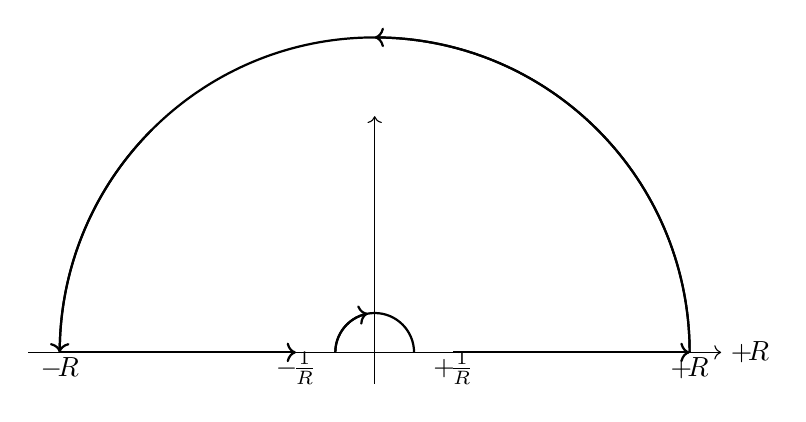
\begin{tikzpicture}[scale=2]
  % Axes
  \draw[->] (-2.2,0) -- (2.2,0) node[right] {$+$\!$R$};
  \draw[->] (0,-0.2) -- (0,1.5);

  % Semicircular arc (upper half-plane)
  \draw[thick, <-] (-2,0) arc (180:135:2);
  \draw[thick] (-2,0) arc (180:0:2);
  \draw[thick, <-] (0,2) arc (90:0:2);
  
  % Small semicircle around origin
  \draw[thick] (-0.25,0) arc (180:0:0.25);
  \draw[thick,->] (-0.25,0) arc (180:100:0.25);

  % Arrows along real axis
  \draw[thick, ->] (-2,0) -- (-0.5,0);
  \draw[thick, ->] (0.5,0) -- (2,0);

  % Labels
  \node at (-2, -0.1) {$-\!R$};
  \node at (-0.5, -0.1) {$-\!\frac{1}{R}$};
  \node at (0.5, -0.1) {$+\!\frac{1}{R}$};
  \node at (2, -0.1) {$+\!R$};
\end{tikzpicture}\]
Prove that 
\[\int_{\Gamma_R}(\frac{e^{iz}}{z} - \frac{1}{z})\,dz = 0.\]
\begin{solution}
    Since $\Gamma_R$ is closed, it suffices, by Cauchy's theorem, to show that $\frac{e^{iz}}{z} - \frac{1}{z}$ is entire on $D_{R + 1}(0).$ Clearly, The function $\in H(D_{R + 1}(0) \sm \{0\}).$ We will show that if we define 
    \[f(z)  = \begin{cases}
        \frac{e^{iz}}{z} - \frac{1}{z}, \quad z\neq 0\\
        i, \qquad \qquad z = 0
    \end{cases},\] then $f$ is continuous at $0$ since
    \[\lim_{z\to 0} f(z) = \lim_{z\to 0} \frac{1}{z}\sum_{n=0}^\infty \frac{(iz)^n}{n!} - \frac{1}{z} = i.\] Since we forgive singularities, we have that $f \in H(D_{R + 1}(0)).$ and so 
    \[\int_{\Gamma_R}(\frac{e^{iz}}{z} - \frac{1}{z}) \, dz = \int_{\Gamma_R}f(z)\, dz = 0.\]
\end{solution}


\newpage
\section*{Problem 2}
\begin{problem}
    Suppose that $\gamma_R(\theta) = Re^{i\theta}, \quad \theta \in [0, \pi]$ is the upper semicricle arc. Show that 
    \[\lim_{R\to \infty}\int_{\gamma_R} \frac{e^{iz}}{z}\,dz = 0\]
\end{problem}
\begin{figure}[H]
    \centering
    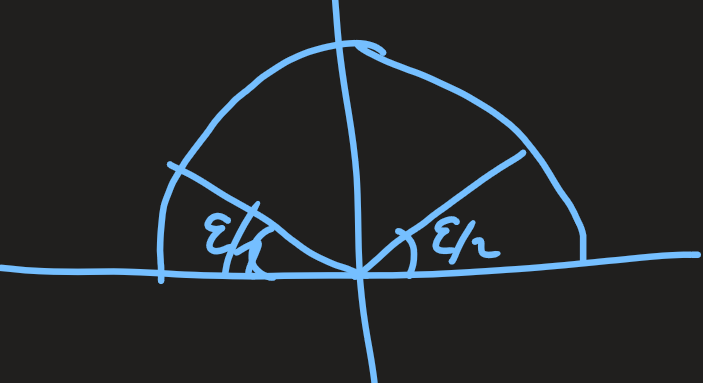
\includegraphics[width=0.5\linewidth]{Images/non-assmnet.png}
\end{figure}
\begin{solution}
Consider the paths in the picture above, where $\gamma_R^{(1)}, \gamma_R^{(3)}$ are the small pizza slices and $\gamma_R^{(2)}$ is the big pizza slice. Thus, 
\begin{align*}
    \left|\int_{\gamma_R} \frac{e^{iz}}{z}\, dz\right| &\leq \left|\int_{\gamma_R^{(2)}} \frac{e^{iz}}{z}\, dz\right| + 2\left|\int_{\gamma_R^{(1)}} \frac{e^{iz}}{z}\, dz\right|\\
    &\leq \text{arclength}\big[\gamma_R^{(2)}\big]\max_{z \in \gamma_R^{(2)}}(|\frac{e^{iz}|}{|z|}) + 2\cdot \text{arclength}\big[\gamma_R^{(1)}\big]\max_{z \in \gamma_R^{(1)}}(|\frac{e^{iz}|}{|z|})\\
    &\leq \pi R \frac{1}{R}\max_{z \in \gamma_R^{(2)}}(|{e^{iz}|}) + \epsilon R \frac{1}{R}\max_{z \in \gamma_R^{(1)}}(|{e^{iz}|})\\
    &= \pi \max_{y \in \gamma_R^{(2)}}({e^{-y}}) + \epsilon \max_{y \in \gamma_R^{(1)}}({e^{-y}})\\
    &= \pi {e^{-R\sin(\frac{\epsilon}{2})}} + \epsilon \\
    &\to \epsilon
\end{align*}

\end{solution}
\newpage

\section*{Problem 3}
\begin{problem}
    Prove that if $\Tilde{\gamma}_R = \frac{1}{R}e^{i\theta},$ $\theta \in [0, \pi],$ then 
    \[\lim_{R\to \infty} \int_{\Tilde{\gamma}_R}(\frac{e^{iz}}{z} - \frac{1}{z}) \, dz = 0 \]
\end{problem}
\begin{solution}
    Again, we estimate
    \begin{align*}
      \left|\int_{\Tilde{\gamma}_R}(\frac{e^{iz}}{z} - \frac{1}{z}) \, dz\right|  &\leq \text{arclength}\big[\Tilde{\gamma}_R\big]\max_{z \in \Tilde{\gamma}_R}(\frac{|e^{iz}|}{|z|} - \frac{1}{|z|})\\
      &= \frac{\pi}{R} \max_{z = \frac{1}{R}}(z + \frac{1}{2}z^2 + \dots)\\
      &\to 0
    \end{align*}
\end{solution}

\newpage
\section*{Problem 4}
\begin{problem}
    Prove that $\int_{-\infty}^\infty \frac{\sin(x)}{x}\, dx = \pi.$
\end{problem}
\begin{solution}
By symmetry, 
\[\int_{-R}^R \frac{\cos(x)}{x}\,dx =  \int_{-R}^R \frac{1}{x}\, dx = 0.\] Thus, by the previous part, we can say that in the limit,
\begin{align*}
    i\int_{-R}^R \frac{\sin(x)}{x}\, dx &= \int_{-R}^R \frac{\cos(x) + i\sin(x)}{x}- \frac{1}{x}\, dx\\
    &= \int_{-R}^R \frac{e^{ix}}{x} - \frac{1}{x}\, dx\\
    &= \int_{\Gamma_R}\frac{e^{iz}}{z} - \frac{1}{z}\, dz - \int_{\gamma_R}\frac{e^{iz}}{z} - \frac{1}{z}\, dz\\
    &= \int_{\gamma_R} \frac{1}{z}\,dz\\
    &= \int_0^\pi \frac{1}{Re^{i\theta}}Rie^{i\theta}\\
    &= i\pi,
\end{align*}
and thus 
\[\int_{-R}^R \frac{\sin(x)}{x}\, dx = \pi\]
    
\end{solution}

\newpage
\section*{Problem 5}
\begin{problem}
    Verify the Cauchy-Riemann equations for 
    \[f(z) = e^{z^2}\]
\end{problem}
\begin{solution}
    ($\frac{\partial u}{\partial x} = \frac{\partial v}{\partial y}$) Note that 
    \[e^{z^2} = e^{2z}= e^{2x + 2iy} = e^{2x}(\cos(2y) + i\sin(2y)) = e^{2x}\cos(2y) + ie^{2x}\sin(2y).\] Thus
    \begin{align*}
      \frac{\partial u}{\partial x}  &=   2e^{2x}\cos(2y)\\
      &= e^{2x}(2\cos(2y))\\
      &= \frac{\partial v}{\partial y}
    \end{align*}
    and 
    \begin{align*}
        \frac{\partial v}{\partial x} &= 2e^{2x}\sin(2y)\\
        &= -(-2e^{2x}\sin(2y))\\
        &= -\frac{\partial u}{\partial y}
    \end{align*}
\end{solution}

\newpage
\section*{Problem 6}
\begin{problem}
    Suppose that $a,b \in \bbC$ with $|a| < r < |b|$ and 
    \[\gamma(\theta) = re^{i\theta}, \quad \theta \in [0, 2\pi].\] Evaluate 
    \[\int_\gamma \frac{1}{(z - a)(z-b)}\, dz.\]
\end{problem}
\begin{solution}
    Consider the function
    \[f(z):= \begin{cases}
        \frac{1}{(z - a)(z-b)} - \frac{1}{(z-a)(a-b)}, \quad z\neq a\\
        \frac{-1}{(a-b)^2}, \qquad \qquad z = a
    \end{cases}\]
    Note that 
\begin{align*}
    \lim_{z\to a} f(z) &= \lim_{z\to a}\frac{1}{(z - a)(z-b)} - \frac{1}{(z-a)(a-b)}\\
    &= \lim_{z\to a} \frac{1}{z-a}\left[\frac{1}{z-b} - \frac{1}{a-b}\right]\\
    &= \lim_{z\to a} \frac{1}{z-a}\left[\frac{a-b - z + b}{(z-b)(b-a)}\right]\\
    &= \lim_{z\to a} \frac{-1}{(z-b)(a-b)}\\
    &= \frac{-1}{(a-b)^2}
\end{align*}. Thus, $f$ is continuous on $z = a.$ Moreover, there exists some $R$ such that $|r| < R < b,$ and thus $f\in H(D_R(0))$ since it forgives $z = a.$ Since $\gamma$ is closed, we have by Cauchy that 
\[\int_\gamma \frac{1}{(z - a)(z-b)} - \frac{1}{(z-a)(a-b)}\, dz = \int_\gamma f(z)\,dz = 0.\] Thus, it suffices to calculate 
\[\frac{1}{a-b}\int_\gamma \frac{1}{z - a}\,dz = \frac{1}{a-b}2\pi i.\] Thus, 
\[\int_\gamma \frac{1}{(z-a)(z-b)}\, dz = \frac{2\pi i}{b-a}\]
\end{solution}

\newpage
\section*{Problem 7}
\begin{problem}
    Suppose $f(z)$ is a nonconstant entire function. Prove that the range of $f$ is dense in $\bbC.$
\end{problem}
\begin{solution}
    Let $z_0\in \bbC.$ Suppose there exists some $r>0$ such that $f(z)\notin B_r(z)$ for any $z\in \bbC.$ Define 
    \[g(z) = \frac{1}{f(z) - z_0}.\] Note that $g \in H(\bbC).$ Note that 
    \[|g(z)| = \frac{1}{|f(z) - z_0|} < \frac{1}{r}.\] Thus, $g(z)$ is constant and so $f(z) - z_0$ is constant and thus $f$ is constant. A contradiction.
\end{solution}

\end{document}